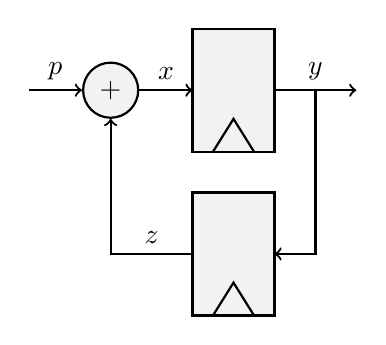
\begin{tikzpicture}[scale=0.52,thick]
    % adder
    \node[circle,draw,minimum size=.7cm,fill=gray!10] (a) at (0,0) {\textred{$+$}};
    \draw[->] (-2,0) --node[above]{\textpurple{$p$}} (a);
    \draw[->] (a) --node[above]{$x$} (2,0);
    % register1
    \draw[fill=gray!10] (2,-1.5) rectangle (4,1.5);
    \draw (2.5,-1.5) -- (3,-0.7) -- (3.5,-1.5);
    \draw[->] (4,0) --node[above]{$y$} (6,0);
    % register2
    \draw[fill=gray!10] (2,-5.5) rectangle (4,-2.5);
    \draw (2.5,-5.5) -- (3,-4.7) -- (3.5,-5.5);
    \draw[->] (5,0) -- (5,-4) -- (4,-4);
    \draw[->] (2,-4) --node[above]{$z$} (0,-4) -- (a);
\end{tikzpicture}
